\documentclass[12pt,titlepage]{article}
\usepackage[english]{babel}
\usepackage[dvipsnames,rgb,dvips,table]{xcolor}
\usepackage{graphicx}
\usepackage[font=small,labelfont=bf]{caption}
\graphicspath{{Figures/}}
\usepackage{psfrag}
\usepackage{dcolumn}
\usepackage{bm}
\usepackage{amsmath}
\usepackage{amssymb}
\usepackage[rflt]{floatflt}
\usepackage{latexsym}
%\usepackage{float}
\usepackage{bm}
\usepackage{subcaption}
\usepackage{booktabs}
\usepackage{floatrow}
\floatsetup[table]{font=footnotesize}
\usepackage{hyperref}
\usepackage{array}
\usepackage{ragged2e}
\usepackage[bottom]{footmisc}
\usepackage{algorithm2e}

\usepackage[left=20mm,right=20mm,top=25mm,bottom=20mm]{geometry}

\author{}
\title{}

%\setlength{\parskip}{3pt}

% QUOTES: `` ''

\begin{document}
%\parindent=0cm


\section*{A genetic algorithm for supply chain optimization}

\subsection*{The (general) mathematical framework}

A set of facilities is placed on a $L \times L$ square space. Each facility can belong to one of $K$ different types, and there are $N_i$ facilities of type $k$, with $i = 1, \ldots, K$. For example, the kinds can be $\lbrace$Customers, Stores$\rbrace$, in which case $K=2$, or $\lbrace$Retailers, Warehouses, Manufacturers$\rbrace$, in which case $K=3$.
Furthermore, each facility of type $1$ (end-customer) is characterised by a (given) scalar value $x_j$, with $j = 1, \ldots, N_1$, representing the facility demand of products. Similarly, facilities of type $K$ (suppliers) are characterised by a (given) scalar value $s_j$, with $j = 1, \ldots, N_K$, representing the supplier output capacity.

Each facility of type $k$ (apart from those of type $K$) can be connected to (at most) one facility of type $k+1$, representing a request of products from that facility. Once connections are determined, we have a weighted $K$-partite graph $G = (F_1, F_2, \ldots, F_K, E)$ which corresponds to the supply-chain network of facility sub-sets $F_1, F_2, \ldots, F_K$, connected by edges set $E$. Edges are weighted, with the weight being the (Euclidean) distance between the connected nodes.

The problem of optimizing the supply chain can therefore be solved by finding a the edges set $E$ that optimizes some objective function measuring the network performance. This objective function can of course be defined in many different ways and we are going to try a few of them. 

An option, possibly the simplest one, is measuring the network performance in terms of the fraction of satisfied end-customers:
\[
f(E) = \dfrac{1}{N_1} \ \sum_{j=1}^{N_1} \theta_j, \quad \mbox{where} \quad \theta_j = \begin{cases} 1 \ \mbox{if} \ \exists i \ \mbox{such that} \ (j,i) \in E \\ 0 \ \mbox{otherwise} \\ \end{cases} \ .
\]

Although very simple to define and evaluate, this objective function is unsuitable for our purposes, as it is independent on edges weights, and therefore on the spacial distribution of the facilities. A more suitable definition of the objective function to optimize is in terms of the supply chain profit. To a first approximation, we will measure the profit as total amount of items sold to end-users minus transportation costs. 
In mathematical terms:
\begin{equation}
f(E) = \sum_{j=1}^{N_1} \theta_j^{[1]} x_j^{[1]} \ - \alpha \ \sum_{k=1}^{K-1} \ \Bigl( \ \sum_{j=1}^{N_k} \theta_j^{[k]} \ x_j^{[k]} \ w_{j*}^{[k]} \ \Bigr) \ ,
\label{eq:fitness}
\end{equation} 
where $\alpha$ is a parameter determining the transportation cost of one unit of product per unit distance and $w_{j*}^{[k]}$ is the weight of the outbound connection (if any) of node $j$ of nodes set $F_k$. Although a bit more complicated, we think that this definition might be more suitable for the goals of our project, one of which is indeed investigating the effect of parameter $\alpha$ on the structure of the best network found by the optimization algorithms that we are going to use.

\subsection*{Side note}
In several relevant articles (e.g.~\cite{altiparmak2006genetic, amiri2006designing, syarif2002study}) the approach is quite different from ours: while these authors start from a given set of potential locations for facilities and design an optimal network, we generate random maps (i.e. random facility locations) and then optimize the structure of the network once the facility locations are determined. Our intention, rather than optimizing a real supply chain by means of real world data and optimization methods, is in fact to create a more abstract model and investigate the role of parameters and the effect of local as opposed to global interactions.

In a later phase of the project, however, we might consider the problem of optimally placing a new facility (e.g. a warehouse) in the space in order to maximise the profit increase.

\subsection*{Supply chain as a generalised assignment problem and GA optimization}

\subsubsection*{2-layers supply chain}

In the simplest case $K = 2$ (two kinds of facilities, i.e. customers and suppliers) the problem described above is equivalent to a generalised assignment problem, a well defined problem in combinatorial optimization. In this problem, quoting Wikipedia, ``there are a number of agents and a number of tasks. Any agent can be assigned to perform any task, incurring some cost and profit that may vary depending on the agent-task assignment. Moreover, each agent has a budget and the sum of the costs of tasks assigned to it cannot exceed this budget. It is required to find an assignment in which all agents do not exceed their budget and total profit of the assignment is maximized.'' 

In our case, clearly, customers correspond to tasks, and suppliers to agents performing the tasks. Costs of tasks/deliveries are the customers' demands and budgets of the agents/suppliers are their supply capacity. The profit obtained by an agent/supplier performing a task/delivery to a customer depends on the distance between the supplier and the customer. In our case, however, the concept of profit is not associated to the agent/supplier, but rather to the job/customer: profits are made by selling products to end-customers, and the sum of all these profits is the measure of the supply chain performance.

Chu and Beasley (REFERENCE) proposed a genetic algorithm approach to solve the generalised assignment problem. See the original paper for encoding and genetic operators specification [of course will be described in the final report].

[TO-DO: Important, describe the concept of unfitness for solving constrained optimization problems]

We have implemented the method described above to find a close-to-optimal network configuration in the simple case $K = 2$, using the fitness function defined in Eq.~\ref{eq:fitness}. The best networks found by the GA for the same map and different $\alpha$ values are shown in in Figure~\ref{fig:GA_0.05} ($\alpha = 0.05$) and \ref{fig:GA_0.3} ($\alpha = 0.3$). In this first simple case, we have 100 customers (blue circles) and 10 suppliers (red triangles) on a $10 \times 10$ square, customers' demands are all equal to 1 and suppliers' capacities are all equal to 10. The effect of $\alpha$ in this simple example is clear and intuitive: if the transportation cost of one unit of product per unit distance is too high, shipping products to customers located too far away from a supplier is unprofitable, and therefore the best solution found by the GA is a disconnected graph, in which many customers are not served. $\alpha$ seems to also play a role in the convergence speed of the algorithm, although this has not been investigated in depth yet (and maybe it is not so interesting).

\begin{figure}[hbtp]
    \centering
    \begin{subfigure}[b]{0.475\textwidth}
        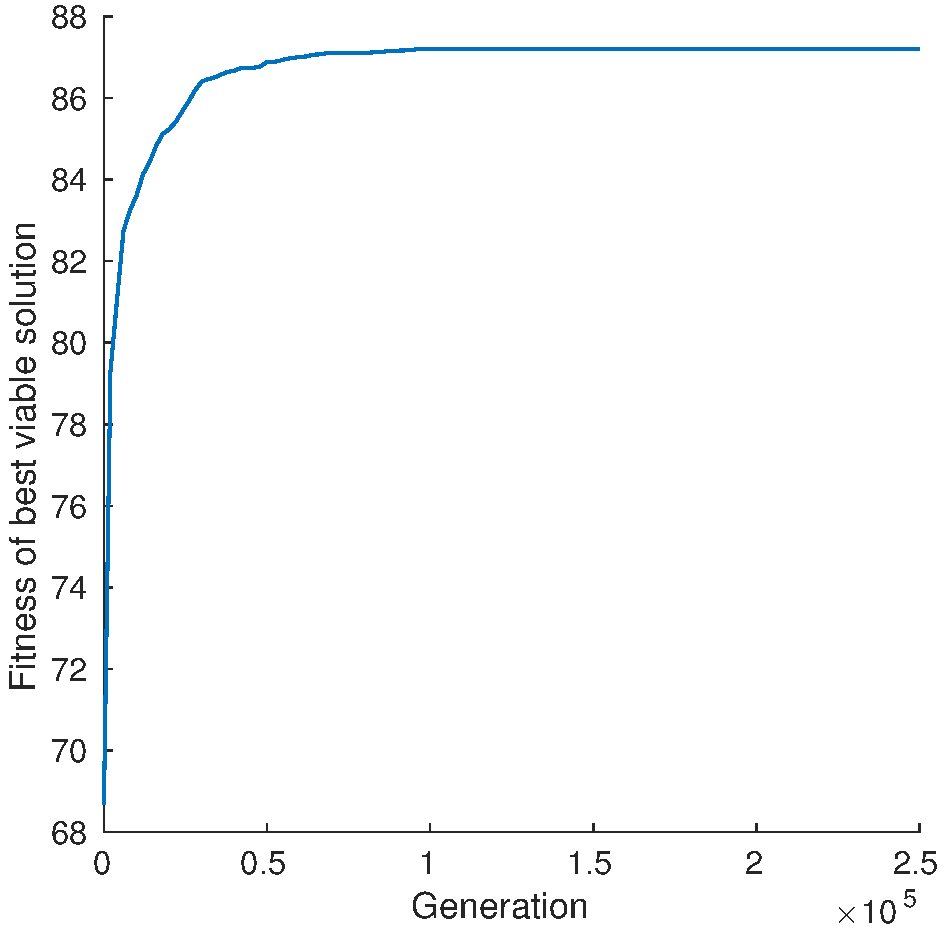
\includegraphics[width=\textwidth]{fitness_2l_005.pdf}
    \end{subfigure}%
    \hfill%
    \begin{subfigure}[b]{0.475\textwidth}
        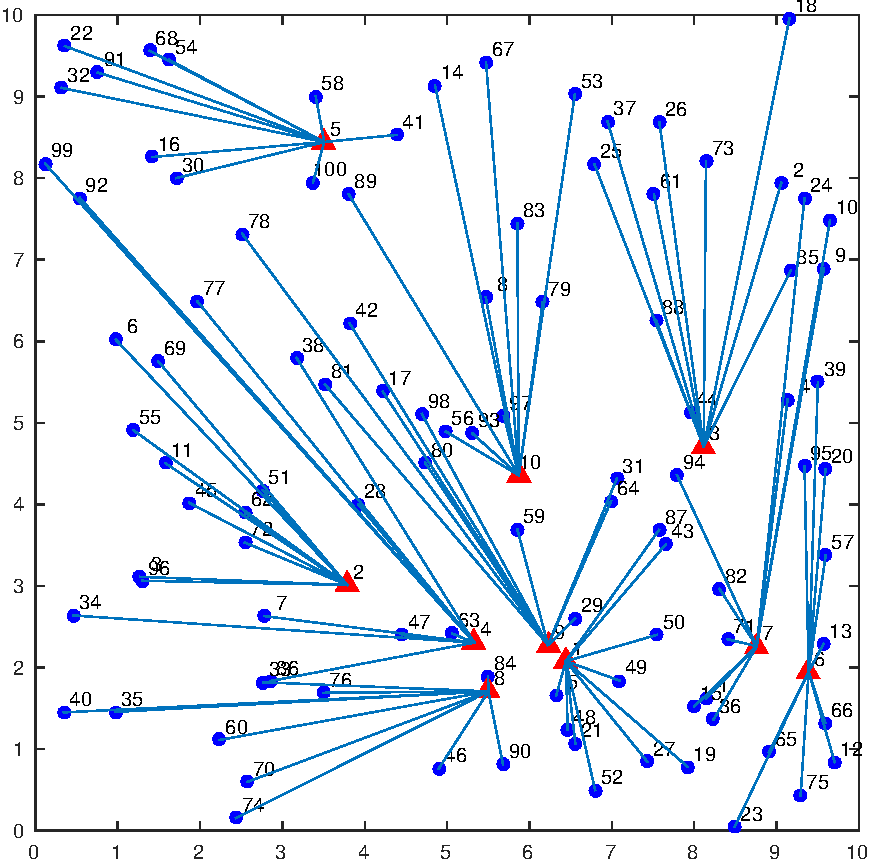
\includegraphics[width=\textwidth]{network_2l_005.pdf}
    \end{subfigure}
    \caption{2-layer supply chain optimized with a GA. Left panel: maximum fitness over generations. Right panel: best network found by the GA. Transportation cost $\alpha = 0.05$.}\label{fig:GA_0.05}
\end{figure}

\begin{figure}[hbtp]
    \centering
    \begin{subfigure}[b]{0.475\textwidth}
        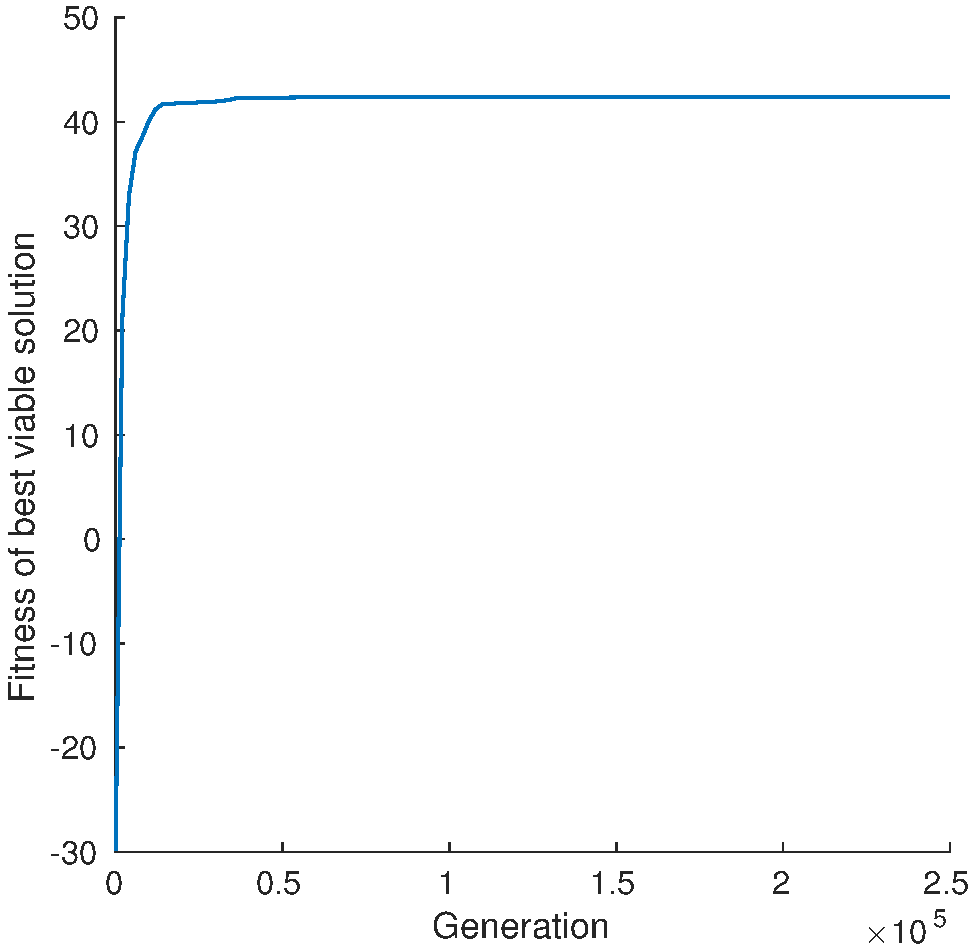
\includegraphics[width=\textwidth]{fitness_2l_03.pdf}
    \end{subfigure}%
    \hfill%
    \begin{subfigure}[b]{0.475\textwidth}
        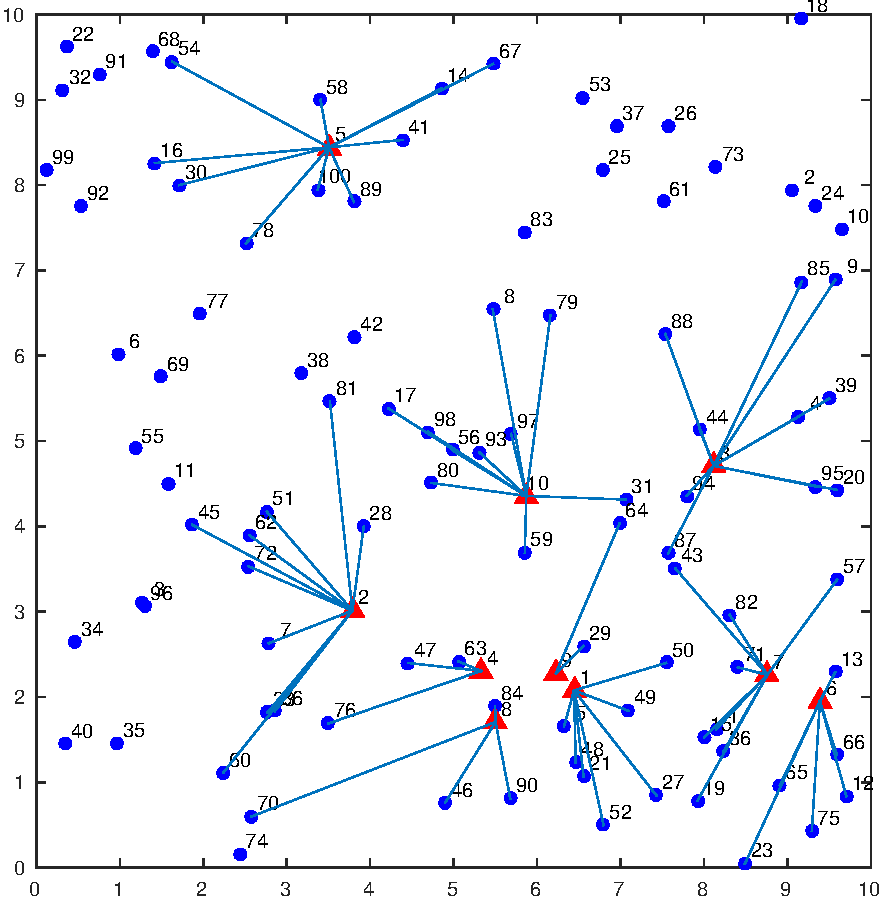
\includegraphics[width=\textwidth]{network_2l_03.pdf}
    \end{subfigure}
    \caption{2-layer supply chain optimized with a GA. Left panel: maximum fitness over generations. Right panel: best network found by the GA. Transportation cost $\alpha = 0.3$.}\label{fig:GA_0.3}
\end{figure}

\subsubsection*{3-layers supply chain}

Although the 2-layer case is simple and equivalent to a well-defined problem in combinatorial optimization, we need at least 3 layers in order to have a nontrivial supply chain model. We tried to generalise the GA approach to deal with a generalised ``multi-assignment''\footnote{This name is to distinguish this problem from the multi-level generalized assignment problem, a different combinatorial optimization problem in which agents can work at multiple levels of efficiency} problem, in which there are several levels of assignment: jobs are assigned to agents at the lowest assignment level, then agents are assigned to upper-level structures, and so on. In our case, with $K=3$, ``retailers'' (level-1 customers) are assigned to  ``warehouses'' (level-1 suppliers), which in turn (as level-2 customers) are assigned to ``manufacturers'' (level-2 suppliers). Note that this problem, which can be generalised to $K$ levels, is \emph{much} harder than the classical generalised assignment problem, as in general it cannot be broken up into multiple problems to solve separately.

We modified the GA proposed by Chu and Beasley to deal with multiple levels of assignment, by encoding the second layer in a second chromosome and allowing the demands of level-2 customers (the warehouses) to be variables, given by the sum, for each warehouse, of the orders of level-1 customers made to that particular warehouse. The GA then works basically as in the simpler 2-layer case, apart from some minor modification to the genetic operators (e.g. crossover now occurs, stochastically, between chromosomes corresponding to the same layer).

[Explain modifications to unfitness]

We present here (Figure~\ref{fig:GA_3l_0.05}) an example with 100 retailers (blue circles), 10 warehouses (green squares) and 2 manufacturers (red triangles), on a $10 \times 10$ square. Demand of all retailers is 1 unit and supply of each manufacturer is 50 units. The transportation cost $\alpha$ here is set to 0.05. In the best network find by the GA (right panel), the flow of items from the manufacturers to the warehouses is represented by red edges of proportional width.

\begin{figure}[hbtp]
    \centering
    \begin{subfigure}[b]{0.475\textwidth}
        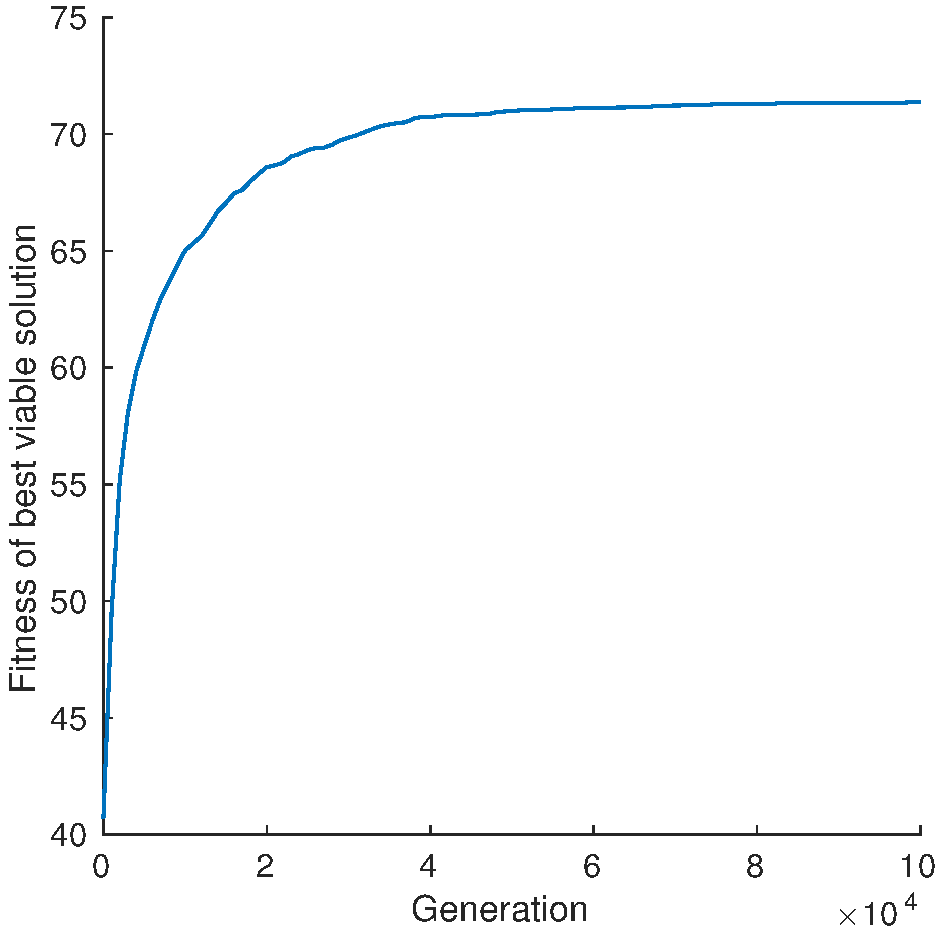
\includegraphics[width=\textwidth]{fitness_3l_005.pdf}
    \end{subfigure}%
    \hfill%
    \begin{subfigure}[b]{0.475\textwidth}
        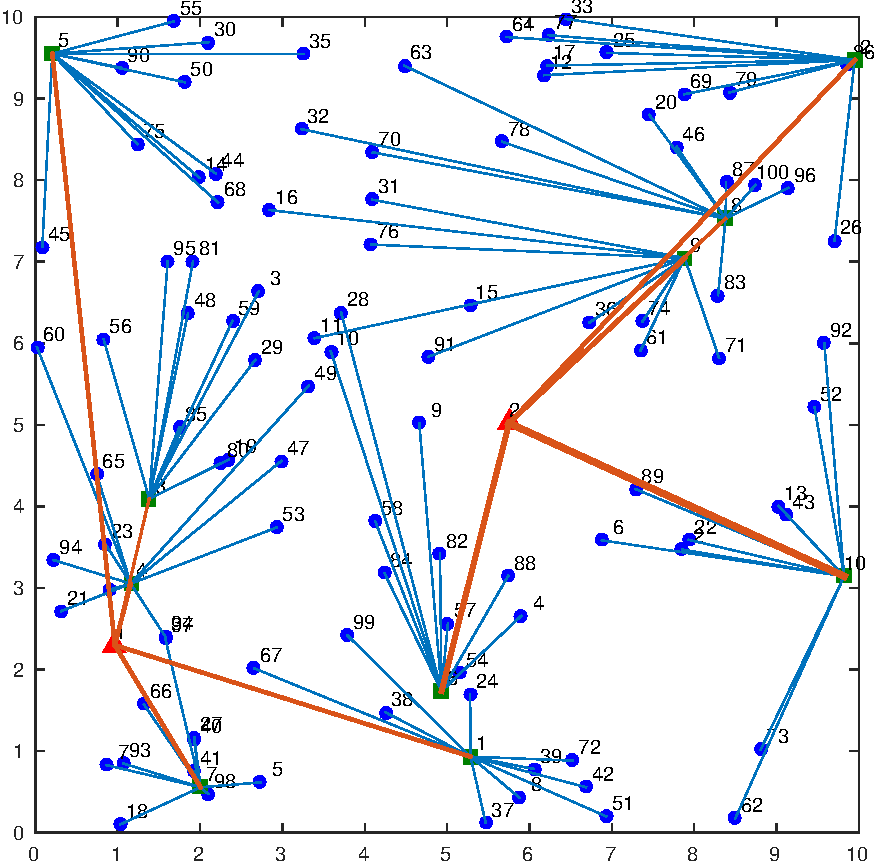
\includegraphics[width=\textwidth]{network_3l_005.pdf}
    \end{subfigure}
    \caption{3-layer supply chain optimized with a GA. Left panel: maximum fitness over generations. Right panel: best network found by the GA. Transportation cost $\alpha = 0.05$.}\label{fig:GA_3l_0.05}
\end{figure}



\bibliography{references} 
\bibliographystyle{abbrv}





\end{document}





